\documentclass[acmsmall,review,nonacm]{acmart}
\usepackage{graphicx} % Required for inserting images
\usepackage{mathpartir}
\usepackage{listings}
\let\Bbbk\undefined
\usepackage{amssymb}
\usepackage{amsmath}
\usepackage{tikz}
\usetikzlibrary{automata, positioning}

\title{Mhira: Message History Invariants for Refining Parametric Actor System Verification}
\author{Christian Fontenot}
\email{christian.fontenot@colorado.edu}
\affiliation{
    \institution{University of Colorado Boulder}
    \city{Boulder}
    \state{Colorado}
    \country{USA}
}

\usepackage{xcolor}
\definecolor{Cayenne}{HTML}{941100}
\definecolor{Mocha}{HTML}{945200}
\definecolor{Asparagus}{HTML}{929000}
\definecolor{Fern}{HTML}{4F8F00}
\definecolor{Clover}{HTML}{008F00}
\definecolor{Moss}{HTML}{009051}
\definecolor{Teal}{HTML}{009193}
\definecolor{Ocean}{HTML}{005493}
\definecolor{Midnight}{HTML}{011993}
\definecolor{Eggplant}{HTML}{011993}
\definecolor{Plum}{HTML}{942193}
\definecolor{Maroon}{HTML}{942193}

\begin{document}
\newcommand{\net}{\mu}
\newcommand{\mkmsg}[5]{(#1,#2)\rightarrow(#3,#4,#5)}
\newcommand{\msg}{m}
\newcommand{\hist}{\omega}
\newcommand{\loc}{\ell}
\newcommand{\progloc}{\texttt{l}}
\newcommand{\exitloc}{\texttt{exit}}
\newcommand{\entryloc}{\texttt{entry}}
\newcommand{\mkloc}[3]{#1.#2.#3}
\newcommand{\evnt}{e}
\newcommand{\addr}{a}
\newcommand{\ty}{t}
\newcommand{\store}{\zeta}
\newcommand{\actstore}{\eta}
\newcommand{\var}{x}
\newcommand{\val}{v}
\newcommand{\cons}[2]{#1\cdot#2}
\newcommand{\mkstate}[4]{\langle\cons{\cons{\textcolor{Plum}{#1}}{\textcolor{Cayenne}{#2}}}{\cons{\textcolor{Teal}{#3}}{#4}}\rangle}

\newcommand{\absaddr}{\hat{\addr}}
\newcommand{\sep}[2]{#1*#2}
\newcommand{\linsep}[2]{#1\otimes#2}
\newcommand{\tool}{\texttt{Mhira}}
\newcommand{\absnet}{\textcolor{Teal}{\hat{\net}}}
\newcommand{\absmsg}{\hat{\msg}}
\newcommand{\mkptp}[5]{(#1,#2)\rightarrow_{P2P}(#3,#4,#5)}
\newcommand{\mkbcast}[5]{(#1,#2)\rightarrow_{BC}(#3,#4,#5)}
\newcommand{\absloc}{\textcolor{Plum}{\hat{\loc}}}
\newcommand{\absstore}{\textcolor{Cayenne}{\hat{\store}}}
\newcommand{\absactstore}{\hat{\actstore}}
\newcommand{\msggraph}{\hat{M}}
\newcommand{\mksymstate}[4]{\langle\cons{\cons{\textcolor{Plum}{#1}}{\textcolor{Cayenne}{#2}}}{\cons{\textcolor{Teal}{#3}}{#4}}\rangle}

% Semantics 
\newcommand{\mktrans}[3]{#1 \mathrel{\mathord{-}\mkern-4mu[#2]\mkern-4mu\mathord{\rightarrow}} #3}
\newcommand{\instrstep}[2]{#1\rightarrow_c#2}
\newcommand{\step}[2]{#1\rightarrow#2}
\newcommand{\eval}[2]{#1\downarrow#2}
\newcommand{\absstep}[2]{#1\rightsquigarrow#2}
\newcommand{\absinstrstep}[2]{#1\rightsquigarrow_c #2}
\newcommand{\abseval}[2]{#1\Downarrow#2}
\newcommand{\code}[1]{\texttt{#1}}


\lstdefinelanguage{P}{
  morekeywords={
    machine, event, fun, var, type, enum, spec, module, test, 
    start, state, entry, exit, on, goto, do, defer, ignore, raise, send, broadcast,
    new, assert, assume, if, else, while, foreach, in, sizeof, return, true, false, null,
    int, seq
  },
  sensitive=true,
  morecomment=[l]{//},
  morecomment=[s]{/*}{*/},
  morestring=[b]",
  morestring=[b]',
  alsoletter={:}
}
\lstset{language=P}

\newcommand{\lstbasicstyle}{\ttfamily\ttfamily\small}
\newcommand{\lstkeywordstyle}{\color{Cayenne}\bfseries}
\newcommand{\lstcommentstyle}{\sl}
\newcommand{\lstnumberstyle}{\scriptsize\em}

\lstdefinestyle{default}{%
  backgroundcolor=\color{white},%
  basicstyle=\lstbasicstyle,%
  commentstyle=\lstcommentstyle,%
  keywordstyle=\lstkeywordstyle,
  numbers=left,
  numberstyle=\lstnumberstyle,
  columns=fullflexible,%
  keepspaces=true,%
  mathescape=true%
}
\lstset{style=default}

\newcommand{\jedi}[1]{\textcolor{blue}{[#1]}}
\begin{abstract}
    Backwards-unrealizability is a tantalizing approach to parametric actor systems verification, as it can reason about only relevant system slices. However, the length of an error witness trace is still unbounded, and so non-determinism can prevent this technique from scaling, even if human intuition says the analysis should stop. 

    Coarse inductive invariants can be used to further prune the search space considered, allowing for backwards-unrealizability based techniques to scale to more realistic systems, without expensive pre-analyses. In this work, we present one such possible coarse invariant over message histories, and define an automaton abstraction capable of capturing the possible behaviors of parametric systems. We illustrate its efficacy on a series of benchmarks written in the P language.
    
\end{abstract}
\maketitle

\section{Introduction}

Safety verification of parametric distributed systems is challenging whether it is approached from a forwards or backwards analysis. In the former case, the number of distinct processes is unknown, and may lead to excessive materialization of processes. In the latter, non-determinism from actor behaviors leads to a state-space explosion, which worsens as the number of message handlers increases, exponentially. This means that although a backwards-from-error may be theoretically enticing, it is held back by challenges of scalability. 

While parametric actor verification is challenging, it is nonetheless an increasingly important programming paradigm, as distributed computation becomes cheaper. Thus, verification of safety is more necessary than ever. Even fundamental protocols such as Paxos\cite{lamport2019part} are as of yet not verified automatically, and most distributed applications ``in the wild'' are built \emph{on top} of these protocols. 

A backwards-from-error approach to safety verification has shown promise in the adjacent area of event-driven systems\cite{meier2023historia}, but its application to parametric programs has been limited, either by restrictions on abstraction\cite{conchon2012cubicle}, or by limitations on practical scale. When transitioning backwards, choosing which process to consider, as well as which handler to consider, produces non-determinism not originally present in the forwards-direction. Lack of pre-analysis can cause a backwards approach to construct traces which are not actually possible under any given configuration, wasting the time of the analyzer in the best case, and in the worst case preventing termination entirely.

Backwards-Unrealizability as an analysis technique relies on transitioning backwards from error, until a fixpoint is computed. If a state is encountered which is contradictory (assuming error), it is removed. We observe that to speed  up the construction of such a fixed point, if we can start with some inductive invariant $\varphi$ characterizing states reachable from initial, we can prune states in the backwards invariant which do not satisfy $\varphi$, as they \emph{cannot} reach initial.

One such invariant we consider is one restricting the set of possible traces. If we had such an invariant, we could detect when an infeasible trace is constructed, and prune the path immediately, saving execution time. 

In this project report, we define a Message History Automaton, which is an automaton which recognizes a superset of all possible traces produced by a parametric actor system. We give an abstract semantics for a subset of the P language\cite{desai2013p} to construct these automata for a protocol, which then allows us to use them in a backwards analysis to accelerate verification. 

Our contributions are as follows: 
\begin{itemize}
    \item We define \emph{Message History Automata} as a coarse over-approximation of the possible message histories produced by parametric actor protocols. 
    \item We define a \emph{symbolic interval domain} to allow the construction of these automata in programs which rely on configuration parameters during runtime. 
    \item We implement a tool to construct these automata, named \tool\, and evaluate whether these automata can be produced quickly.
\end{itemize}

\section{Overview}

\subsection{Computing Message History Invariants}
We will illustrate the construction of message history invariants via Two-Phase Commit, a core distributed systems protocol for agreement. The language we will be analyzing is P\cite{desai2013p}, a modeling language for message passing systems (simplified to reduce noise and focus on our contributions).

In brief, a P program is a set of actors (keyword \texttt{machine}), which contain message handlers defining how they react to events. We assume each actor to have an initial event, which they start by receiving and executing.

Two-Phase commit begins with a coordinator  and a set of Participants (code shown in Figure \ref{fig:coord}). The coordinator begins by broadcasting a proposed value to all participants in the system. Each participant will then respond positively if they have not already agreed on a value to commit. If every participant responds in this way, then the coordinator broadcasts a command to commit the proposed value to memory.

While Two-Phase commit is conceptually quite simple, in practice reasoning about its safety is non-trivial, as an unbounded number of processes need to be considered, and concurrency further complicates this.

One way to simplify reasoning is to pre-compute coarse inductive invariants on message histories, to reduce the number of execution interleavings which need to be explored to prove safety. To do this, we define a pre-analysis which computes an invariant $\phi$, which can be leveraged by a more detailed analysis.

States in our abstraction are made up of 4 components: a distributed location map $\absloc$, which maps actor addresses to program locations, a distributed store $\absstore$ which maps addresses to local stores $\hat{\eta}$, a network $\absnet$ which is a multiset of in-flight messages, and a message history automaton $\msggraph$. 

The automaton contains a vertex for each event handler in the program, and weighted, directed edges between the two. Each edge contains 2 weights: a weight $(a,b)$ from $v_1$ to $v_2$ means the handler $v_1$ can send in total $b$ copies of $v_2$ to the system, while to a single actor it will send $a$ copies (thus, $b$ must be at least equal to $a$).

\begin{figure}
\begin{minipage}{0.48\textwidth}
\begin{lstlisting}
machine Coordinator {
    var nodes: Pars; var received: int; 
    var acc: bool;
    on eInitial do (i:CoordInit) {
        nodes = i; 
        received = 0;
        broadcast nodes, eProp, 5;
    }
    on eResp do {
        var par: Participant;
        received = received + 1;
        if (received >= sizeof(nodes)){
            broadcast nodes, eFinal;
        }
    }
}
\end{lstlisting}
\end{minipage}
\hspace{1em}
\begin{minipage}{0.48\textwidth}
    \begin{lstlisting}[firstnumber=17]
machine Participant {
    var internal: int; var potential: int;
    var coord: Coordinator;
    on eInit do (c: Coordinator) {
        internal = -1;
        coord = c; 
        potential = -1;
    }
    on eProp do (z : int) {
        potential = z;
        if (internal == -1){
            send coord, eResp;
        }
    }
    on eFinal do {
        assert potential != -1;
        internal = potential;
    }
}   
\end{lstlisting}
\end{minipage}
    \caption{P Source code for Two phase commit. We assume a single Coordinator, and $k$ Participants.}
    \label{fig:coord}
\end{figure}

We begin our symbolic execution with a simple initial state:
each machine type in the program has a ``canonical actor'' representing it during the abstract execution, and they start at the top of their initial message handlers. The network begins empty. Our message automaton starts with 5 vertices (one per handler), and no edges (as no messages have been sent). 

Symbolic execution of the participant's initial message does not affect our network at all, instead simply setting fields, so we omit discussion of it. During the execution of \texttt{eInitial}, the analysis encounters a broadcast to all participants, with value 5. This adds a broadcast message to the network, which we distinguish from point-to-point messages.\par 

Upon all actors reaching the end of their handlers, we consider the network to decide what to do next. As there is only one message, we choose it, and deliver it. In doing so, besides updating stores and locations, we update our automaton as follows: 

As the message is a \emph{broadcast}, the pairwise weight between \texttt{eInitial} and 
\texttt{eProp} is incremented by 1 (from 0), and the system weight is incremented by $k$, the number of Participants globally. In Figure \ref{fig:graphone}, we show the current automaton state, which has only this edge. 

\begin{figure}[h]
    \centering
    \scalebox{0.75}{
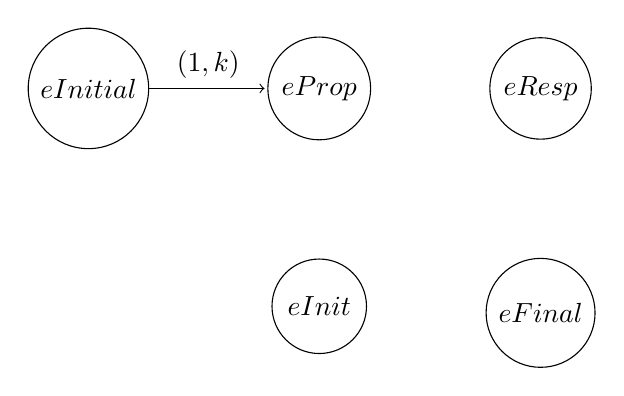
\begin{tikzpicture}[shorten >=1pt,node distance=1.5cm,every state/.style={minimum size=1.2cm}]
    \node[state] (q0) {$eInitial$};
    \node[state] (q1) [right=of q0] {$eProp$};
    \node[state] (q2) [right=of q1] {$eResp$};
    \node[state] (q3) [below=of q1] {$eInit$};
    \node[state] (q4) [below=of q2] {$eFinal$};
    \path[->] (q0) edge node[above] {$(1,k)$} (q1);
\end{tikzpicture}
}
    \caption{Our message history automaton after receiving \code{eProp}}
    \label{fig:graphone}
\end{figure}

Now, we begin the execution of \code{eProp}. After setting \code{potential}, we reach the condition on line 27. Since we have not yet seen an assignment to internal which may make this false, the (vacuous) else branch cannot occur. On line 28, we encounter a send of $eResp$ to a coordinator $coord$, adding the \emph{point-to-point} message to the network.\par 

Reaching the end of the handler, we are again at a point where both canonical actors are idle, and must again choose a message from the network. We can only choose the just-added $eResp$, accordingly updating the location and store of our coordinator. Now, we consider updating our automaton $\msggraph$: 

As the pairwise in-degree of \code{eProp} is 1, we produce the pairwise weight $1*1 = 1$, as there is a single send occurring. For the system-wide weight, the handler occurs $k$ times, and each sends a single message, so we get $k*1 = k$, producing the updated automaton in Fig \ref{fig:graphtwo}.

\begin{figure}
    \centering
    \scalebox{0.75}{
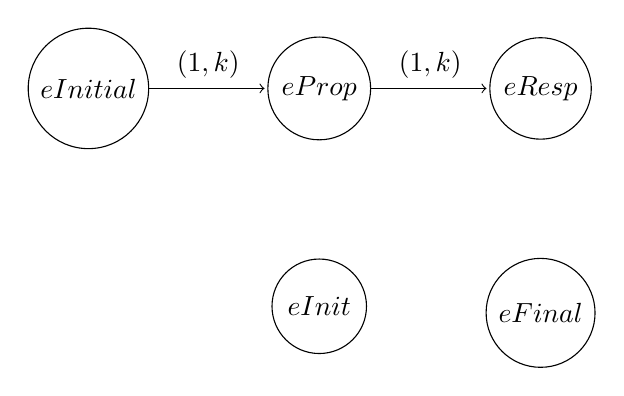
\begin{tikzpicture}[shorten >=1pt,node distance=1.5cm,every state/.style={minimum size=1.2cm}]
    \node[state] (q0) {$eInitial$};
    \node[state] (q1) [right=of q0] {$eProp$};
    \node[state] (q2) [right=of q1] {$eResp$};
    \node[state] (q3) [below=of q1] {$eInit$};
    \node[state] (q4) [below=of q2] {$eFinal$};
    \path[->] (q0) edge node[above] {$(1,k)$} (q1);
    \path[->] (q1) edge node[above] {$(1,k)$} (q2);
\end{tikzpicture}}
    \caption{Updated automaton after receiving \code{eResp}}
    \label{fig:graphtwo}
\end{figure}

We can now consider the execution of \code{eResp}. The field \code{received} is incremented, then we compare it to our symbolic constant $k$. As we cannot know if $1 \ge k$ without a concrete $k$, we split, and consider both options. In the else case, no messages are sent, and the graph stays unchanged. For the true case, a broadcast is sent to all Participants, of event \code{eFinal}. In this case, we would similarly add the edge with weight $(1,k)$ to our graph, however this is insufficient. This is a single execution of the handler, and we know from the in-degree of our vertex that $k$ executions occur total. From our system parameters, we know there to be a single \code{Coordinator} actor, so we multiply the weights in our edge by $(total/(\#Coordinator) = k/1 = k$, yielding the weight $(k,k^2)$. This produces the message history automaton shown below:\\

\begin{center}
\scalebox{0.75}{
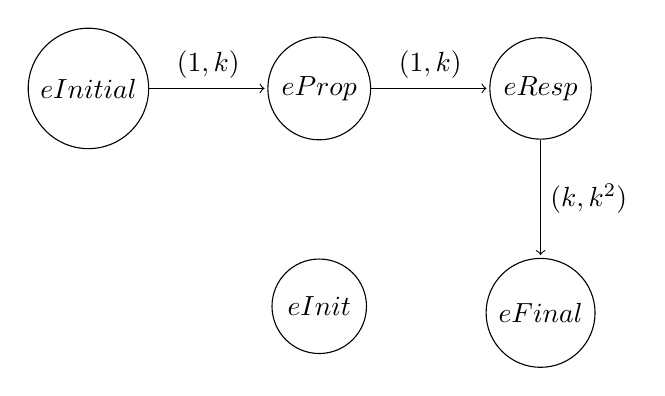
\begin{tikzpicture}[shorten >=1pt,node distance=1.5cm,every state/.style={minimum size=1.2cm}]
    \node[state] (q0) {$eInitial$};
    \node[state] (q1) [right=of q0] {$eProp$};
    \node[state] (q2) [right=of q1] {$eResp$};
    \node[state] (q3) [below=of q1] {$eInit$};
    \node[state] (q4) [below=of q2] {$eFinal$};
    \path[->] (q0) edge node[above] {$(1,k)$} (q1);
    \path[->] (q1) edge node[above] {$(1,k)$} (q2);
    \path[->] (q2) edge node[right] {$(k,k^2)$} (q4);
\end{tikzpicture}}
\end{center}


We now have two states at the same program location, and can join them. They differ only in the automaton, where one has the new edge and the other does not, so the automaton with all three edges is the result of our join. Finally, we can execute \code{eFinal}, which does not send any messages, and our analysis is complete after this, returning the above automaton. 

An astute reader may raise a complaint about our message automaton: With infinite precision, we should have our third edge be $(1,k)$ as well, as only 1 execution of \code{eResp} will actually have the message be sent. We leave the refinement of this to future work, as this requires finer-grained reasoning about symbolic arithmetic. 

\subsection{Using the Automaton Invariant}

Now that we have computed an automaton, what does it tell use about possible traces in our system? While a large amount of ordering information is lost, some remains, and we have numeric bounds on the executions of message handlers. 

One property we can assert is the affine-ness of \code{eProp} and \code{eResp}. We define affinity of a message to mean that a given pair of actors can have a message with this event exactly once, which our pair-wise bound denotes. More generally, our pair-wise bound restricts how many times a specific pair of abstract actors may communicate. 

Our system-wide bound also restricts the space of possible histories: We know from our graph that only $k$ copies of \code{eProp} can be sent globally within the system, so any analysis should never consider the possibility of more than $k$ occurring. Additionally, we know that our history is bounded by length $k+k+k^2$, as they are the sum of the system-wide bounds along all paths in the graph.

As a final piece of information, we have some causal constraints maintained in our automaton: A feasible message history containing a message corresponding to a vertex $v$ requires that a message for a vertex with an edge to $v$ precede it in the message history. In our example, this means a history cannot have \code{eInitial}, and then \code{eResp}, with no \code{eProp} in-between. In this manner, our graph structure is effectively a symbolic weighted-DFA encoding the shape of valid histories, using weights to bound length. 

\subsection{Ring Example}

Now that we have illustrated the use of our abstraction on a protocol like Two-Phase Commit, let us also illustrate its behavior for cyclical protocols such as ring-based algorithms. 

\begin{figure}
    \centering
    \begin{lstlisting}
machine Node {
    var id: int; var succ: Node;
    var leader: bool;
    on eInit do (c:Config){
        id = c.id;
        succ = c.succ;
        leader = false;
        send succ, eFwd, id;
    }
    on eFwd do (v: int){
        if (v > id){
           send succ, eFwd, v;
        } else if (v == id){
            leader = true;
        }
    }
}
\end{lstlisting}
    \caption{A simple leader election protocol for rings.}
    \label{fig:changrobert}
\end{figure}

Figure \ref{fig:changrobert} defines a simple protocol for electing a leader in a ring: Each node has a successor, and an id. Each node forwards its id to its successor. When an id is received, if it is larger than the node's, it forwards it again. When a node receivers its own id it becomes the leader. 

As in Two-Phase Commit, we start our abstraction with a single canonical Node, at the beginning of \code{eInit}. We use $n$ to denote the number of nodes. Executing \code{eInit}, the canonical actor sends a single \code{eFwd}. Adding this to the automaton, we get the following: 

\begin{center}
\scalebox{0.75}{
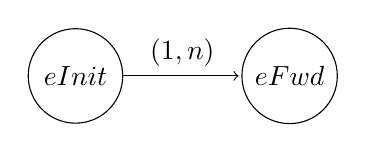
\begin{tikzpicture}[shorten >=1pt,node distance=1.5cm,every state/.style={minimum size=1.2cm}]
    \node[state] (q0) {$eInit$};
    \node[state] (q1) [right=of q0] {$eFwd$};

    \path[->] (q0) edge node[above] {$(1,n)$} (q1);
\end{tikzpicture}}
\end{center}

Now, we execute \code{eFwd}, branching on our condition as before (all ids have unknown value). In the true branch, a message to \code{eFwd} is sent. As before, this is a single send, so a self-loop with weight $(1,n)$ is added:  

\begin{center}
\scalebox{0.75}{
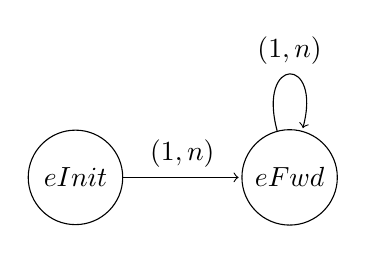
\begin{tikzpicture}[shorten >=1pt,node distance=1.5cm,every state/.style={minimum size=1.2cm}]
    \node[state] (q0) {$eInit$};
    \node[state] (q1) [right=of q0] {$eFwd$};

    \path[->] (q0) edge node[above] {$(1,n)$} (q1);
    \path[->] (q1) edge[loop above] node {$(1,n)$} ();
\end{tikzpicture}}
\end{center}

As there is another send to \code{eFwd}, we repeat the process: 

\begin{center}
\scalebox{0.75}{
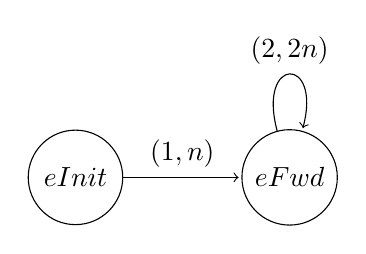
\begin{tikzpicture}[shorten >=1pt,node distance=1.5cm,every state/.style={minimum size=1.2cm}]
    \node[state] (q0) {$eInit$};
    \node[state] (q1) [right=of q0] {$eFwd$};

    \path[->] (q0) edge node[above] {$(1,n)$} (q1);
    \path[->] (q1) edge[loop above] node {$(2,2n)$} ();
\end{tikzpicture}}
\end{center}

After incrementing an edge a set number of times (in our case, 5), we can simply widen both numbers to $\infty$, producing a final automaton:

\begin{center}
\scalebox{0.75}{
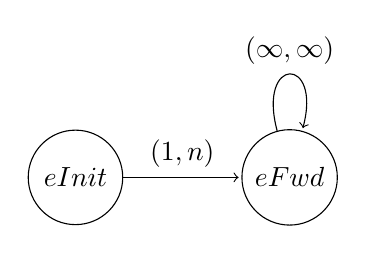
\begin{tikzpicture}[shorten >=1pt,node distance=1.5cm,every state/.style={minimum size=1.2cm}]
    \node[state] (q0) {$eInit$};
    \node[state] (q1) [right=of q0] {$eFwd$};

    \path[->] (q0) edge node[above] {$(1,n)$} (q1);
    \path[->] (q1) edge[loop above] node {$(\infty,\infty)$} ();
\end{tikzpicture}}
\end{center}

This gives us a very coarse invariant over message histories, one which we hope to refine in future work. In particular, the infinite edge weights illustrate an interesting challenge in cyclic protocols for symbolic execution, as history can be arbitrarily long. More precise abstractions for symbolic constant arithmetic may again be useful here in providing stricter bounds. \par 

\section{Concrete Domain and Semantics}

As a basis for our abstract semantics we begin with a brief definition of our concrete system. 

\subsection{Concrete System}

We define a state in our system to be the 4-tuple $\mkstate{\loc}{\store}{\net}{\hist}$.

\begin{itemize}
    \item $\loc$ is a map from actor addresses $a$ to program locations. 
    \item $\store$ is a map from actor addresses $\addr$ to local stores $\eta$, which map variables to values.
    \item $\net$ is a set of sent but undelivered messages. 
    \item $\hist$ is an ordered list of received messages.
\end{itemize}

Collectively, a state thus contains information about the current locations and states of actors, alongside the network, and a history of what has happened so far in execution.

We define an actor address as an unspecified type $\addr$, and an actor location as the triple $\mkloc{\ty}{\evnt}{\progloc}$, noting the actor's type, current event under execution, and program location within the event handler. We denote special program locations $\entryloc$ and $\exitloc$ to denote the beginning and end of a handler, respectively.

We define an actor's store $\eta$ to be a map from variables $\var$ to values $\val$. The domain of values is left parametric to our system, though we assume actor addresses and sets of values to be included in this domain.

As our analysis is focused on messages and setting bounds on them, it is worth discussing in more depth what information a message carries, as we carry additional information to maintain soundness later. In a minimal interpreter, a message needs an event label, a receiver, and an argument. We further add in a sender address, as well as the sending event / location. This means our history tracks not just that an actor received a message, but even where in the program it was sent \emph{from}.

With messages defined, we can define the network $\net$ as a multiset of currently in-flight messages, and a message history $\hist$ as an ordered list of delivered messages. We note that the message history is not strictly necessary for execution. 

\begin{figure}
\begin{mathpar}
\inferrule[Step-Instr]{\mktrans{\progloc}{c}{\progloc'} \in \pi(\ty)(\evnt) 
\quad \instrstep{\eta}{\eta'}}
{\step{\mkstate{\addr\mapsto(\mkloc{\ty}{\evnt}{\progloc}),\loc}{\addr\mapsto\eta,\store}{\net}{\hist}}{\mkstate{\addr\mapsto(\mkloc{\ty}{\evnt}{\progloc'}),\loc}{\addr\mapsto\eta',\store}{\net}{\hist}}} \and 
\inferrule[Step-Send]{
\mktrans{\progloc}{send\ y,\evnt',v}{\progloc'} \in \pi(\ty)(\evnt) \quad 
\eval{(v,\eta)}{w}\quad \eval{(y,\eta)}{\addr'} \quad \msg = (\addr,\addr',\evnt',w)
}{
\step{\mkstate{\addr\mapsto\mkloc{\ty}{\evnt}{\progloc},\loc}{\store}{\net}{\hist}}
{\mkstate{\addr\mapsto\mkloc{\ty}{\evnt}{\progloc'},\loc}{\store}{\net,\msg}{\hist}}}
 \and 

 \inferrule[Step-Broadcast]{\mktrans{\progloc}{broadcast\ \ty',\evnt',v}{\progloc'} \in \pi(\ty)(\evnt) \quad 
\eval{(v,\eta)}{w}\quad  \quad \net' = \bigcup_{\addr_i\mapsto\mkloc{\ty}{\cdot}{\cdot} \in \loc} (\addr,\addr_i,\evnt',w)
}{\step{\mkstate{\addr\mapsto\mkloc{\ty}{\evnt}{\progloc},\loc}{\store}{\net}{\hist}}
{\mkstate{\addr\mapsto\mkloc{\ty}{\evnt}{\progloc'},\loc}{\store}{\net\cup\net'}{\hist}}}
\and 
\inferrule[Step-Handle]{
\msg = (\addr',\addr,\evnt',v) \quad \texttt{on\ $\evnt'$\ do (x)\{$\cdots$\}}\in \pi(\ty) \quad dropLocals(\eta)[x\mapsto v] = \eta'
}{
\step{\mkstate{\addr\mapsto\mkloc{\ty}{\evnt}{\exitloc},\loc}{\addr\mapsto\eta,\store}{\net,\msg}{\hist}}{\mkstate{\addr\mapsto\mkloc{\ty}{\evnt'}{\entryloc},\loc}{\addr\mapsto\eta',\store}{\net}{\hist;\msg}}
}

\end{mathpar}
\caption{Concrete semantics of the distributed actor system. We note that Step-Instr is defined along some parametric instruction language, rather than defining loops, conditionals, and more ourselves.}
\label{fig:conc}
\end{figure}


With our domains well-defined, we give a concrete semantics in Figure \ref{fig:conc}. Besides the parametric \texttt{Step-Instr} rule, we have 3 actor-specific constructs to reason about: send, broadcast, and handle.\par 

When a send statement is encountered, the address expression is evaluated to find the sender, the arguments are evaluated, and then a message is added to the network. Broadcast works almost exactly the same, but creates a message for each actor of the specified type, instead of just one. 

Message delivery is handled by \texttt{Step-Handle}. If an actor is currently idle (at $\exitloc$ for some event), and a message is addressed to it, we can deliver it, removing it from the network, and adding it to the message history. The receiving actor moves to the start of the corresponding event, and has its store updated. We define a helper function $dropLocals(\actstore)$ to remove all fields which were local to the previous handler, and then extend the resulting store with any parameters to the new handler.\par 

\section{Message Reachability Invariants}\label{sec:absem}

\subsection{Abstract Domain}

\begin{mathpar}
        \text{locations}\quad \mkloc{\ty}{\evnt}{\progloc} \quad\quad 
        \text{distributed\ locations}\quad \absloc ::= \epsilon\ |\ \sep{\absaddr\mapsto\mkloc{\ty}{\evnt}{\progloc}}{\absloc} \\ 
        \text{stores}\quad \hat{\eta} ::= \epsilon\ |\ \sep{x\mapsto\hat{v}}{\hat{\eta}}\quad \quad \text{distributed\ stores}\quad \absstore ::= \epsilon\ |\ \sep{\absaddr\mapsto\hat{\eta}}{\absstore}\\
        \text{messages}\quad \absmsg ::= \mkptp{\addr_s}{\evnt_s}{\addr_r}{\evnt_r}{\hat{v}}\ |\ \mkbcast{\addr_s}{\evnt_s}{\ty}{\evnt_r}{\hat{v}}\quad\quad \text{networks }\quad \absnet ::= \varepsilon\ |\ \linsep{\absmsg}{\absnet} \\
        \text{message graph} \quad \msggraph \quad\quad \text{abstract states}\quad \alpha ::= \mksymstate{\absloc}{\absstore}{\absnet}{\msggraph}
    
\end{mathpar}
We define an abstraction of our concrete domain which is suitable for capturing bounds on message sends, as a 4-tuple,mirroring the concrete domain: $\mksymstate{\absloc}{\absstore}{\absnet}{\msggraph}$. We apply a structural abstraction in the vein of \cite{van2010abstracting} for the first three components:

$\absloc$ is a separation logic formula capturing the location of some set of actors. We interpret our separation logic formulae intuitionistically, allowing for only some actors in the concrete system to be needed in the abstract. 

Similarly, $\absstore$ is a separation logic formula capturing their stores. We define an individual actor's store abstraction $\absactstore$ to again be a separation logic formula, with the value abstraction $\hat{v}$ left as a parameter to the analysis. This parameterization allows for increased or decreased precision as necessary to capture stronger bounds. In principle, mapping all values to $\top$ is equivalent to removing all state-based context, allowing only a syntactic check of our ``may-send'' property.

For messages $\absmsg$, we define two constructs, distinguishing whether a message is sent by broadcast or as a single (peer-to-peer) message. This allows the analysis to distinguish a case which the standard concrete semantics does not: If a network contains two messages $\msg_1$ and $\msg_2$, which differ only in the receiver's address, were the two sent by broadcast, or by two distinct \code{send} commands? As our parametric abstraction will consider a finite number of abstract actors, we must distinguish whether a delivered message may correspond to many (broadcast) or not. For a broadcast, rather than a receiving address, we consider a receiving type.

Networks $\absnet$ become a linear logic formula containing abstract messages $\absmsg$, which in turn are piecewise abstractions of the concrete message $\msg$: addresses become symbolic, and values are abstracted as in the stores.\par 

We define message graphs in Figure \ref{fig:msggraph}. 
Vertices in the message graph are pairs of actor types $T$ and events $e$, allowing us to distinguish receipt of messages by actors of distinct types. Edges are directed, and weighted by two numeric abstract values. The edge $((T_1,e_1),(T_2,e_2),(a,b))$ is interpreted as: an actor of type $T_1$ may send an actor of type $T_2$ the event $e_2$ at most $a$ times from its handler for $e_1$, and will send $b$ in total (differs due to broadcast messages).

\begin{figure}
\begin{mathpar}
    \msggraph ::= (V,E) \quad V \subseteq (T,Ev) \quad E \subseteq (V\times V\times \hat{\mathbb{N}}\times\hat{\mathbb{N}}) \\ 

    Ev ::= idle \vert \cdots  \quad T ::= main \vert \cdots
\end{mathpar}
\caption{Definition of a message graph $\msggraph$, which is a graph of vertices consisting of type,event pairs, with edges weighted by two upper bounds on send counts, one recording pairwise sends, and the other recording system-wide sends.}
\label{fig:msggraph}
\end{figure}

\subsection{Message History Automata}

Formally, the message graph can be thought of as an automaton, a notion we define now as it is useful in expressing its relation to concrete histories. A Message History Automaton $\msggraph$ is a tuple $(V,I,\hat{\mathbb{N}},\delta)$, where we define $V$ as the set of vertices above, $I \subseteq V$ as the set of initial states, $\hat{\mathbb{N}}$ is a numeric abstraction, and $\delta \subseteq V\times\ V\times((\hat{\mathbb{N}},\hat{\mathbb{N}})\cup \varepsilon)$ describes the edges of our graph, with additional epsilon edges. We do not define accepting states, as every state in the automaton is accepting, since ``may-reach'' is an over-approximation. 

The $\varepsilon-$edges of our transition relation can be thought of as ``reset'' transitions: as we over-approximate possible histories, it is possible for a message chain to simply stop instead of executing in full. Formally, the only edges with this weight are those from states in $V$ to states in $I$.

\subsection{Abstract Semantics}

With our abstract states defined, we can now define an abstract semantics which allows us to capture message history invariants. 

\begin{figure}
    \centering
    \begin{mathpar}
\inferrule[Abs-Instr]{\absinstrstep{\hat{\eta}}{\hat{\eta}'}
    \quad \mktrans{\progloc}{c}{\progloc'} \in \pi(\ty)(\evnt) }
    {\absstep{\mksymstate{\sep{\absaddr\mapsto(\mkloc{\ty}{\evnt}{\progloc})}{\absloc}}{\sep{\absaddr\mapsto\absactstore}{\absstore}}{\absnet}{\msggraph}}{\mksymstate{\sep{\absaddr\mapsto(\mkloc{\ty}{\evnt}{\progloc'})}{\absloc}}{\sep{\absaddr\mapsto\absactstore}{\absstore'}}{\absnet}{\msggraph}}} \and 

    \inferrule[Abs-Send]{\mktrans{\progloc}{send\ y,\evnt',v}{\progloc'} \in \pi(\ty)(\evnt) \quad 
\abseval{(v,\absactstore)}{\hat{w}}\quad \abseval{(y,\absactstore)}{\absaddr'} \quad \absmsg = \mkptp{\absaddr}{\evnt}{\absaddr'}{\evnt'}{\hat{w}}}{
\absstep{\mksymstate{\sep{\absaddr\mapsto(\mkloc{\ty}{\evnt}{\progloc})}{\absloc}}{\sep{\absaddr\mapsto\absactstore}{\absstore}}{\absnet}{\msggraph}}{\mksymstate{\sep{\absaddr\mapsto(\mkloc{\ty}{\evnt}{\progloc'})}{\absloc}}{\sep{\absaddr\mapsto\absactstore}{\absstore}}{\linsep{\absmsg}{\absnet}}{\msggraph}}
} \and 
 \inferrule[Abs-Broadcast]{\mktrans{\progloc}{broadcast\ \ty',\evnt',v}{\progloc'} \in \pi(\ty)(\evnt) \quad 
\abseval{(v,\absactstore)}{\hat{w}}\quad  \quad \absmsg = \mkbcast{\absaddr}{\evnt}{\ty'}{\evnt'}{\hat{w}}
}{\absstep{\mksymstate{\sep{\absaddr\mapsto(\mkloc{\ty}{\evnt}{\progloc})}{\absloc}}{\sep{\absaddr\mapsto\absactstore}{\absstore}}{\absnet}{\msggraph}}{\mksymstate{\sep{\absaddr\mapsto(\mkloc{\ty}{\evnt}{\progloc'})}{\absloc}}{\sep{\absaddr\mapsto\absactstore}{\absstore}}{\linsep{\absmsg}{\absnet}}{\msggraph}}}

\end{mathpar}
    \caption{Abstract semantics of send and broadcast, alongside parametric instruction language. These are constructed by simply applying our abstractions to the existing concrete rules.}
    \label{fig:structuralabs}
\end{figure}

In Figure \ref{fig:structuralabs}, we define the abstract semantics of commands which are not related to our message history abstraction. These follow simply from our concrete rules, but with concrete components replaced with abstract analogues. Of more interest are the semantics of message delivery, complicated by both the distinction of broadcast and send, and the automaton structure of our message graph.

\begin{mathpar}
    Cfg: \pi\rightarrow T \rightarrow \mathbb{N}\\

    \inferrule[Abs-Handle-P2P]{\absmsg = \mkptp{\absaddr}{\evnt}{\absaddr'}{\evnt'}{\hat{w}} \quad getEdge(\ty,\evnt,\ty',\evnt',\msggraph) = (a,b) \\
    (c,d) = (a+1,b+1*Cfg(\pi)(\ty)) \quad \msggraph' = updateEdge(\ty,\evnt,\ty',\evnt',\msggraph, (c,d))  \quad \texttt{on\ $\evnt'$\ do (x)\{$\cdots$\}}\in \pi(\ty') \\ dropLocals(\absactstore)[x\mapsto \hat{w}] = \absactstore'
    }{
    \absstep{\mksymstate{\sep{\absaddr'\mapsto\mkloc{\ty'}{\evnt''}{\exitloc}}{\absloc}}{\sep{\absaddr'\mapsto\absactstore}{\absstore}}{\linsep{\absmsg}{\absnet}}{\msggraph}}{\mksymstate{\sep{\absaddr'\mapsto\mkloc{\ty'}{\evnt'}{\entryloc}}{\absloc}}{\sep{\absaddr\mapsto\absactstore'}{\absstore}}{\absnet}{\msggraph'}}
    }

    \inferrule[Abs-Handle-BCast]{\absmsg = \mkbcast{\absaddr}{\evnt}{\ty'}{\evnt'}{\hat{w}}
    \quad getEdge(\ty,\evnt,\ty',\evnt',\msggraph) = (a,b) \\
    (c,d) = (a+1,b+Cfg(\pi)(\ty')*Cfg(\pi)(\ty)) \\ \msggraph' = updateEdge(\ty,\evnt,\ty',\evnt',\msggraph, (c,d)) 
    \quad \texttt{on\ $\evnt'$\ do (x)\{$\cdots$\}}\in \pi(\ty') \\ dropLocals(\absactstore)[x\mapsto \hat{w}] = \absactstore'}
    {
    \absstep{\mksymstate{\sep{\absaddr'\mapsto\mkloc{\ty'}{\evnt''}{\exitloc}}{\absloc}}{\sep{\absaddr'\mapsto\absactstore}{\absstore}}{\linsep{\absmsg}{\absnet}}{\msggraph}}{\mksymstate{\sep{\absaddr'\mapsto\mkloc{\ty'}{\evnt'}{\entryloc}}{\absloc}}{\sep{\absaddr\mapsto\absactstore'}{\absstore}}{\absnet}{\msggraph'}}
    }

    
\end{mathpar}

Each rule affects network, locations, and stores in the expected way. Of more significant interest is the effect on the automaton. Let us first consider \code{Abs-Handle-P2P}. Suppose the existing weight corresponding to the message type (senders and receivers) is $(a,b)$. As this is the send of a single message, the first weight, which we use to track pair-wise communication bounds, is incremented by 1.  as that many The latter weight, total communication bounds, is more interesting: The constant factor denotes how many actors of the sending type exist, as each one may send the message once, for a total of $1*Cfg(\pi)(\ty)$ messages in the history. 

The case is similar for broadcast, except that we multiply the total weight by another constant factor, denoting the total number of possible receivers for the message. In this way, we're able to keep track of two weights of interest: how many times can a pair of actors keep communicating, and how many times can the global system witness these messages with different pairs of actors. The former gives us a local view of messages, while the latter is more useful in bounding the total history length. 

When either edge weight is symbolic, an analysis of the system will need to over-approximate some cyclic behavior in order to terminate soundly. This can be helpful in guiding an analysis to unroll multiple executions, or know that it is not possible to unroll (if we need to unroll infinitely). 

\subsection{Join and Widen} 

Given that parametric actor systems model potentially infinite behaviors, it is necessary for termination to define join and widen operations for our semantics. 

To define either, we must first define \emph{when} to join or widen. In particular, each actor in the abstraction has its own location, so two states are only at the same distributed location when all actors agree on location. This is possible only because we have a finite number of actors, and do not grow this set ever. If we were to extend to support adding new actors, we then need to define location equality again, as some may be indirectly comparable. 

Given two actors in the same location, we can define the join $\sqcup$ for the two in a piece-wise manner. To join two distributed stores, we join the stores of each actor, knowing each actor to exist in both because the location also must have each one. To join two actor stores, we start by taking all the mappings which are in one store but not the other. For mappings in both, when we have $x\mapsto\hat{v}$ and $x\mapsto\hat{w}$, we take their join: $x\mapsto(\hat{v}\sqcup\hat{w})$. This value level join is again left as part of the parametric value abstraction, of which we discuss a concrete choice when discussing our evaluation.

Joining two networks is simply the union of as they are sets. Lastly we consider joining two message graph automata. An automaton consists of a set of vertices, and a set of edges. To join two automata, we start with the union of vertices, to get a new vertex set. As we never add vertices this never grows the set. For edges, we follow an approach similar to stores. Any edges in one automaton but not the other are taken, and for edges in both, we take the max of the bounds of each. Our bounds are numbers, or symbolic expressions. To join two numbers, we can simply take the max. For symbolic expressions, one possible max is $\top$ or $\infty$, but we can also choose to take the sum of the two bounds, knowing both must be natural numbers.


\textbf{Widen} is defined analogous to our join, as the piecewise widen of our components. Stores take mappings which are missing in one, and the value-level widen for fields in both. Network widening is defined as the join, as we attempt to guarantee convergence based on the message graph, noting that networks may be an issue in practice. In theory, we could construct protocols $\pi$ where the network grows arbitrarily before being reduced, and this could be an issue for termination. In practice, we have not observed this effect as of yet. Message-graph widening is the same as join, except in taking the max of bounds. If bounds are different, we widen to $\infty$, as it upper bounds any natural number. This widen allows our tool to handle ring algorithms, which would otherwise join infinitely often. This also allows the tool to establish the possible existence of a ring-like structure, as cycles in the graph are the only possible cause of this widen. 

\subsection{Concretization and Soundness}

Having given concrete and abstract domain, we define a concretization relation connecting the two, and use this to show the soundness of our abstract semantics. Connecting abstract and concrete addresses is a valuation map $\theta$.\\ \par 


We begin by detailing the concretization of the message graph automaton, as it is the least direct of our relations. Our formal automaton description of this component now becomes relevant: A concrete message history $\hist$ is concretized by $\msggraph$ if and only if the history corresponds to some string in $L(\msggraph)$, the set of all runs accepted by the automaton. Thus, it is sufficient to describe how to convert a history into a run of the automaton.

Given a message history automaton, $\epsilon$ is always in the concretization relation. For a history $\msg,\hist$, it is in the concretization of $\msggraph$ if and only if we are able to decrement the secondary edge weight corresponding to $\msg$, resulting in a non-zero weight, and starting from the target of that edge, we recurse with $\hist$ as the new history to consider. An additional condition is to check the primary edge weights: for each edge $E$ with weight $(n,m)$, the number of messages corresponding to the edge with the same sender-receiver pair must be at most $n$.

\jedi{Formalizing this in a non-automaton manner is actually really awkward, I've given it a shot but it's clunky.}
We formalize this intuition below: 

\begin{mathpar}
    \epsilon\vDash_\theta\msggraph \\ 
    \mkmsg{\addr}{\evnt}{\addr'}{\evnt}{\cdot},\hist \vDash_\theta\msggraph 
    \iff decrement_\theta(\msggraph, \mkmsg{\addr}{\evnt}{\addr'}{\evnt}{\cdot}) = (n,\msggraph') \land n \ge 0 \land \hist\vDash_\theta\msggraph'
\end{mathpar}

We define $decrement_\theta$ to be an auxiliary function taking a message, and the automaton. Semantically, it is assumed to take the edge corresponding to the message, grab the second weight on the edge, and decrement it by 1, returning both the new weight and the updated graph. Thus, for each message, a total weight is decremented, and as long as this never goes negative the automaton run continues. \par 

The store and location abstractions follow intuitionistic separation logic for their concretization, as follows:\newline 

$\begin{array}{ccl}
     \addr\mapsto\mkloc{\ty}{\evnt}{\progloc},\loc\vDash_{\theta}\sep{(\absaddr\mapsto\mkloc{\ty}{\evnt}{\progloc})}{\absloc} & \iff & \loc\vDash_{\theta}\absloc \quad\text{and}\quad \theta(\absaddr)=\addr\\
     \addr\mapsto\eta,\store\vDash_{\theta}\sep{\absaddr\mapsto\hat{\eta}}{\absstore}\ & \iff & \eta\vDash_{\theta}\hat{\eta} \quad\text{and}\quad \store\vDash_{\theta}\absstore \quad\text{and}\quad \theta(\absaddr)=\addr\\
\end{array}
$

In summary, a distributed location or store models its abstract equivalent under some mapping $\theta$ if and only if there is a concrete actor $\addr$ whose location matches, and has its store model the abstract store, for each abstract actor $\absaddr$ in the symbolic state, such that $\theta(\absaddr)=\addr$. 

As we distinguish between peer-to-peer and broadcast messages, message concretization is slightly indirect: peer-to-peer messages concretize to a single concrete message, while broadcast messages concretize to a set of concrete messages.

$\begin{array}{ccl}
    \mkmsg{\addr}{\evnt_s}{\addr'}{\evnt_r}{w}\vDash_\theta \mkptp{\absaddr}{\evnt_s}{\absaddr'}{\evnt_r}{\hat{w}} & \iff & \theta(\absaddr) = \addr_s \land \theta(\absaddr') = \addr' \land w\vDash_\theta\hat{w}   \\
    \mkmsg{\addr}{\evnt_s}{\addr'}{\evnt_r}{w},\overline{m}\cdot\loc\vDash_\theta \mkbcast{\absaddr}{\evnt_s}{\ty'}{\evnt_r}{\hat{w}} & \iff & \theta(\absaddr) = \addr \land w\vDash_\theta\hat{w}  \land \addr'\mapsto\mkloc{\ty'}{\cdot}{\cdot} \in \loc \land \overline{m}\cdot\loc\vDash_\theta \mkbcast{\absaddr}{\evnt_s}{\ty'}{\evnt_r}{\hat{w}}\\
\end{array}$

As broadcast messages are to a type, rather than specific actors, the location map is needed in the concretization relation in order to ensure the concrete message is to an actor of the same type. We can then define network concretization as a subset relation: $\absnet$ is modeled by $\net$ if each abstract message in $\absnet$ corresponds to some concrete message (or a set, for broadcast) in $\net$.

At the top level, then, an abstract state is modeled by a concrete state if there exists a single mapping $\theta$ of abstract actors to concrete ones such that each individual relation holds.

We can now define a soundness condition for our abstraction, for which we provide an informal proof sketch.

\begin{theorem}[Local Soundness]
If $\sigma\vDash_\theta\hat{\sigma}$ and $\step{\sigma}{\sigma'}$, then there exists $\hat{\sigma}'$ such that $\absstep{\hat{\sigma}}{\hat{\sigma}'}$ and $\sigma'\vDash_{\theta'}\hat{\sigma}'$.
\end{theorem}

\textbf{Informal Argument:} Due to the structural abstraction, the primary rule of interest in establishing soundness is \code{Step-Handle}, as this leads to a non-trivial change to the abstraction. Here, an actor moves location and updates its store, the network removes a single message $\msg$, and adds it to the end of its history $\hist$.

In the abstraction, we have two possible scenarios: the message $\msg$ could be modeled by a broadcast message $\absmsg$, or a peer-to-peer message. In the latter case, we apply \code{Abs-Handle-P2P}, which updates the store, location, and network just as in the concrete system. The message history automaton $\msggraph$ is updated by incrementing the associated edge by $(1,1*Cfg(\pi)(\ty))$, where $\ty$ is the type of the sender. This updates the language recognized by the automaton, by incrementing both bounds by at least 1, safely updating the automaton to recognize the new message. 

In the case of a broadcast, the same edge is incremented by $(1,1*Cfg(\pi)(\ty)*Cfg(\pi)(\ty'))$, adding $1$ to the edge per receiver of matching type. This is always at least one, so it is a sound over-approximation. Future messages from the same broadcast can be safely ignored, as there are in total $Cfg(\pi)(\ty')$ such messages, which has already been accounted for.\par 

\section{Implementation and Evaluation}

We implement our semantics as an abstract interpreter \tool, which produces a set of message history invariants based on the upper bounds of received messages for each actor type in the system. The tool is implemented in F\#, and analyzes a subset of the P language.\par 

\subsection{Value-Level Abstraction}: In our formalism, we have left value level abstractions $\hat{v}$ parametric. To implement the tool in practice, we must pick concrete abstractions. 

We choose to abstract tuples, booleans, integers, actor addresses, and sets of actor addresses, as the allowed values within our program. A tuple is simply a finite set of abstract values, recursively defined. For boolean values we use a simple flat lattice as our domain. Actor addresses are symbolic variables, and sets of them simply refer to all actors of that type. 

Integers prove to be an interesting challenge. An initial approach to integer abstraction may be the interval domain, which  while sound is extremely imprecise, and causes an issue with parametric systems. The protocol $\pi$, written in P, is able to refer to the size of sets of actors. Thus, as our sets are all actors of a given type, the size of a set may be symbolic (as in Two-Phase Commit, and many common protocols). This is a fundamental problem for parametric system analysis To get around this, we construct a \emph{symbolic interval domain} in Figure \ref{fig:symint}, in which interval bounds themselves may be symbolic. For instance, $[0,k]$ is a symbolic interval where $k$ is an unknown natural number. This complicates traditional operations for intervals, as $[1,1] + [0,k]$ should be $[1,k+1]$, and we cannot simplify $k+1$. Thus, we add symbolic addition and multiplication to our domain. This allows for complex intervals like $[r,k+r]$ where $r$ and $k$ are both symbolic. 

Comparison operations on this domain are also complex, and incredibly imprecise. $[1,1] >= [k,k]$ is always $\top$, as we cannot know if $k$ is bigger or not. Symbolic arithmetic further complicates this. For our implementation we fall back on significant imprecision, recognizing that a more precise symbolic arithmetic domain would significantly help the tool, something we leave as future work.

\begin{figure}
\begin{mathpar}
    N ::= \mathbb{Z} | x | N + N | N * N\\ 
    I ::= Int(N,N) | Int(N,\infty) | Int(\infty, N) | \top | \bot\\ 
\end{mathpar}
\caption{The symbolic interval domain. We represent numbers as integers, or symbolic arithmetic using variables $x$. We then use this to define the interval domain as normal.}
\label{fig:symint}
\end{figure}

\subsection{Implementation Details}

We have not yet extended this work to accelerate existing abstract interpreters for the P language, and as such can only provide some cursory empirical results on whether the tool works or not. We have run the tool on 5 benchmarks, as the supported subset is quite limited syntactically, a restriction we intend to quickly lift in future work. We collect data on the time and states explored, to verify that the tool is indeed efficient at building coarse invariants. 

\begin{table}
    \centering
    \begin{tabular}{| c | c | c | c | c |}
         \hline 
         Benchmark & Lines & Handlers & States Explored & Wall-Time (ms)\\
         \hline 
         One-Shot & 38 & 3& 19 & 852\\ 
         Two-Phase Commit & 52 & 5 & 22 & 847\\ 
         Chang-Roberts & 19 & 2 & 12 & 857 \\ 
         Bakery & 94 & 8 & 23 & 854\\ 
         Signal-Barrier & 43 & 6 & 12 & 799 \\
         \hline
    \end{tabular}
    \caption{Preliminary results for message history invariant construction. The number of explored states is smaller than expected, this is due to aggressive joining flattening the invariant size. It would be insightful to either join less often, getting a more precise invariant, or track how many joins and widens actually occur. }
    \label{tab:prelim}
\end{table}

\section{Related Work}

\textbf{Parametric Model Checking:}

In \cite{goel2021symmetry}, the authors consider explicitly the use of symmetry in reducing the state-space explosion latent in message-passing systems. Particularly, this is leveraged to build a symmetry-aware IC3\cite{bradley2012understanding}, which allows for the verification of safety. Unlike our case, this approach attempts to prove safety in full, rather than acceleration. However, the detection of symmetry is used in the same manner, allowing for more knowledge of the system to be gained with less effort, leveraging group theory and the formula representation. We theorize this technique could be used alongside our automaton, to further restrict histories, and it may be possible to augment the automaton itself to learn symmetries.\par 

Cubicle\cite{conchon2012cubicle} is a parametric model checker based on symbolic backward reachability. Cubicle represents its symbolic state as a cube, which is a formula of the shape $\exists \overline{x}. \phi\land\psi$, where $\phi$ is a conjunction of disequalities and $\psi$ is a conjunction of literals. This restricts the representation in a non-trivial manner, and can lead to imprecision. We prefer a more program-state oriented representation, which allows us to explicitly encode additional information during analysis which may help with establishing invariants or unreachability. Our approach should be capable of speeding up Cubicle and related techniques, as well.

\textbf{Message-Passing Systems:} Mailbox abstractions have been considered as a way to capture a similar property of interest, namely bounding the length of an actor's mailbox \cite{stievenart2017mailbox}. While we do not represent mailboxes explicitly, the network in our model is the union of said mailboxes, without ordering (similar to \cite{garoche2008static}). In particular, our message-graph abstraction is a combination of the bounded multiset and graph abstractions described in \cite{stievenart2017mailbox}.\par 

In \cite{meyer2008boundedness}, the author considers the $\pi-calculus$, which is known to map 1-to-1 with actor systems, and attempts to define a bounding on message depth. Our technique similarly attempts to bound depth, with infinite-cycles showing that such a bound could not be established, possibly due to imprecision. Rather than a syntactic flattening, we attempt to establish bounds via abstraction of message communication.\par 

\textbf{Automaton Abstractions:} In \cite{dams2005automata}, the authors propose the use of tree automata as a basis for abstraction, allowing the encoding of hyper-properties and liveness properties. They propose this as a response to the challenge of non-determinism in complex Kripke structures, a challenge which mirrors those raised by concurrency. We handle concurrency via disjunction and joins, which can lose precision, while maintaining a simpler structure. 

The message graph automaton we construct can be viewed as a variant of \emph{symbolic finite automata}\cite{d2017power}, where our guard conditions are simple counters rather than complex predicates. Extending our guard conditions to include boolean comparisons against symbolic constants may reduce the imprecision encountered in our examples.

Visibly pushdown automata\cite{vpa} have been proposed as a model for individual actor processes in actor systems verification \cite{babic2013asynchronously}. This allows for automata-theoretic results to be used in simplification of the parametric model checking problem, but restricts the behaviors of these processes as well. We choose to not restrict, but lose many convenient properties due to this.\par 

Linear-Temporal Logic has been used as a way to restrict the feasible traces of event-driven systems\cite{meier2023historia}. This is the closest work to our own, as we leverage the same goal of restricting feasible traces, though we do not use LTL to do so. Additionally, we do not assume any formulae restricting the trace, but we instead attempt to construct them. Given a closed system, this approach may be leveraged to establish LTL formulae, or other classes of automata, a promising direction.\par  

\textbf{Context-Sensitivity:} The addition of sender information to our messages in both the concrete and abstract systems allows for a more context-sensitive analysis. This idea has been explored in the context of function calls\cite{khedker2008efficiency}\cite{pnueli1981two}, where call-string depth can be useful in constructing paths to refine analysis. In our case, we have effectively length-1 call strings, and so our analysis of a handler is quite insensitive, which is not reflected by our benchmarks' relative simplicity. Scaling the analysis to larger, more realistic systems may require longer-length call-strings, especially if handlers are reused for multiple protocols. 

Concurrency sensitivity\cite{schwarz2024digest} is a recently proposed notion built on the idea of trace partitioning\cite{mauborgne2005trace}. In the latter, it is proposed to consider distinct paths through control-flow structures as distinct executions, rather than naively joining states. This sensitivity can be extended to concurrent programs, and has been explored in representing different thread interleaving contexts. This could be adapted to the actor framework, in particular as a way to further separate calling contexts for handlers, and even to establish symmetries in order to reduce analysis effort.\par 

\section{Future Work}

Automata are a promising direction for coarse invariants to accelerate verification. A purely syntactic check of an actor program produces a coarse message history automaton, and a symbolic execution using a fairly imprecise value abstraction is sufficient to produce numeric bounds on the history. An interesting next step is to consider whether additional information can be added with similar amounts of effort, as experiments show the automaton construction to be very cheap, especially when compared to state-of-the-art verification engines for the full safety problem. 

Symbolic intervals are a necessary piece of our abstraction to handle parametric systems, but they produce significant imprecision during analysis. A future direction which may be promising is to try adding symbolic arithmetic to other traditionally numeric domains, in order to achieve precision. Understanding more fully this relation between symbolic and numeric abstraction is key to improving performance in the area. While we constructed the symbolic interval domain from first principles, work already exists with respect to symbolic ranges\cite{sankaranarayanan2007program}, so we could look to develop a more precise domain, or hopefully leverage existing symbolic + numeric domains. 

We hope as our next steps to incorporate message history automata into existing abstract interpretation frameworks, to evaluate if this is indeed a promising direction of acceleration for some properties. We recognize that it is a cheap invariant to compute, and could reduce goal-directed analysis challenges significantly. 

\bibliographystyle{ACM-Reference-Format}
\bibliography{ref}
\end{document}
